\documentclass[14pt,dvipsnames]{beamer}

\usetheme{Montpellier}
\usecolortheme{beaver}

\usepackage{physics}
\usepackage{amsmath, amssymb, ../../vimacros, hyperref, tikz}
\usetikzlibrary{positioning, fit, bayesnet, shapes.misc, patterns}
\usepackage[round]{natbib}
\usepackage{mathalfa}
\usepackage{cancel}
\usepackage{verbatim}

\beamertemplatenavigationsymbolsempty

\hypersetup{breaklinks=true, colorlinks=true, linkcolor=blue, urlcolor=blue, citecolor=blue}

\newcommand{\balert}[1]{\textcolor{blue}{#1}}
\newcommand{\galert}[1]{\textcolor{PineGreen}{#1}}

\pgfdeclarepatternformonly{stripes}
{\pgfpointorigin}{\pgfpoint{.4cm}{.4cm}}
{\pgfpoint{.4cm}{.4cm}}
{
	\pgfpathmoveto{\pgfpoint{0cm}{0cm}}
	\pgfpathlineto{\pgfpoint{.4cm}{.4cm}}
	\pgfpathlineto{\pgfpoint{.4cm}{.2cm}}
	\pgfpathlineto{\pgfpoint{.2cm}{0cm}}
	\pgfpathclose
	\pgfusepath{fill}
	\pgfpathmoveto{\pgfpoint{0cm}{0.2cm}}
	\pgfpathlineto{\pgfpoint{0cm}{.4cm}}
	\pgfpathlineto{\pgfpoint{0.2cm}{.4cm}}
	\pgfpathclose
	\pgfusepath{fill}
}

\newcommand\Wider[2][3em]{%
\makebox[\linewidth][c]{%
  \begin{minipage}{\dimexpr\textwidth+#1\relax}
  \raggedright#2
  \end{minipage}%
  }%
}

\makeatletter
\newenvironment{noheadline}{
    \setbeamertemplate{headline}{}
    \addtobeamertemplate{frametitle}{\vspace*{-0.9\baselineskip}}{}
}{}
\makeatother

\title{Automatic Differentiation Variational Inference}
\author{Philip Schulz and Wilker Aziz\\
\url{https://github.com/philschulz/VITutorial}}
\date{}

\setbeamertemplate{footline}[frame number]

\begin{document}

\begin{frame}
\maketitle
\end{frame}



\begin{frame}{What we know so far}
    \begin{itemize}
        \item DGMs: \pause probabilistic models parameterised by neural networks \pause
        \item Objective: \pause lowerbound on log-likelihood (ELBO) \pause
        \begin{itemize}
        		\item \alert{cannot be computed exactly} \\ \pause
        		\textcolor{blue}{we resort to Monte Carlo estimation} \pause		
	\end{itemize}
	\item \alert{But the MC estimator is not differentiable} \pause		        
	\begin{itemize}
       		\item Score function estimator: applicable to any model  \pause
		\item Reparameterised gradients\\
		so far seems applicable only to Gaussian variables
        \end{itemize}
    \end{itemize}
    
\end{frame}

\frame{\tableofcontents}


\section{Multivariate calculus recap}

\begin{frame}{Multivariate calculus recap}

Let $x \in \mathbb R^K$ and let $\mathcal T: \mathbb R^K \to \mathbb R^K$ be differentiable and invertible
\begin{itemize}
	\item $y = \mathcal T(x)$
	\item $x = \inv{\mathcal T}(y)$
\end{itemize}

\end{frame}

\begin{frame}{Jacobian}

	The Jacobian matrix $\jac{\mathcal T}{x} $ of  $\mathcal T$ \\
	~assessed at $x$ is the matrix of partial derivatives
	\begin{equation*}
		J_{ij} = \pdv{y_i}{x_j} 
	\end{equation*} 
	
	\pause
	Inverse function theorem
	\begin{equation*}
		\jac{\inv{\mathcal T}}{y} = \left( \jac{\mathcal T}{x} \right)^{-1}
	\end{equation*}
	
\end{frame}

\begin{frame}{Differential (or inifinitesimal)}

	The {\bf differential} $\dd x$ of $x$ \\
	~ refers to an \emph{infinitely small} change in $x$\\ \pause
	\vspace{10pt}

	We can relate the differential $\dd y$ of $y = \mathcal T(x)$ to $\dd x$ \pause
	\begin{itemize}
		\item Scalar case
		\begin{equation*}
			\dd y = \alert{\mathcal T'(x)} \dd x = \alert{\dv{y}{x}} \dd x = \alert{\dv{x}T(x)} \dd x
		\end{equation*}
		where \alert{$\dv*{y}{x}$} is the \emph{derivative} of $y$ wrt $x$ \pause
		\item Multivariate case
		\begin{equation*}
        			\begin{aligned}
			        \dd y = \alert{\djac{\mathcal T}{x}} \dd x % = \alert{\abs{\pdv{x}T(x)}} \dd x % in some texts people will find this notation
		        	\end{aligned}
	        	\end{equation*}
		the absolute value absorbs the orientation 
	\end{itemize}

\end{frame}

\begin{frame}{Integration by substitution}	
	We can integrate a function $g(x)$ \\
	~ by substituting $x = \inv{ \mathcal T}(y)$
	\begin{equation*}
	\begin{aligned}
		\int g(\balert{x}) \alert{\dd x} \pause &= \int g(\underbrace{\balert{\inv{\mathcal T}(y)}}_{x}) \underbrace{\alert{\djac{\inv{\mathcal T}}{y} \dd y}}_{\dd x} \\ \pause
	\end{aligned}
	\end{equation*}
	
	\vspace{-10pt}
	and similarly for a function $h(y)$
	\begin{equation*}
	\begin{aligned}
		\int h(\balert{y}) \alert{\dd y} \pause &= \int h(\balert{\mathcal T(x)}) \alert{\djac{\mathcal T}{x} \dd x}
	\end{aligned}
	\end{equation*} 

\end{frame}

\begin{frame}{Change of density}

Let $X$ take on values in $\mathbb R^K$ with density $p_X(x)$\\ \pause
~ and recall that $y = \mathcal T(x)$ and $x = \inv{\mathcal T}(y)$\\ \pause

~

Then $\mathcal T$ induces a density $p_Y(y)$ expressed as
\begin{equation*}
p_Y(y) = p_X(\inv{\mathcal T}(y)) \djac{\inv{\mathcal T}}{y}
\end{equation*} \pause
and then it follows that
\begin{equation*}
p_X(x) = p_Y(\mathcal T(x)) \djac{\mathcal T}{x}
\end{equation*}

	
\end{frame}

\section{Reparameterised gradients revisited}

\begin{frame}{Revisiting reparameterised gradients}
	Let $Z$ take on values in $\mathbb R^K$ with pdf $q(z|\lambda)$ \\
	
	~ \pause

	The idea is to count on a \emph{reparameterisation} \\ \pause
	~ a transformation $\mathcal S_\lambda: \mathbb R^K \to \mathbb R^K$ such that \pause
	\begin{equation*}
	\begin{aligned}
	\mathcal S_\lambda(z) &\sim \pi(\epsilon) \\ \pause
 	\inv{\mathcal S}_\lambda(\epsilon) &\sim q(z|\lambda) \pause
	\end{aligned}
	\end{equation*} 
	\begin{itemize}
		\item $\pi(\epsilon)$ does not depend on parameters $\lambda$\\
		we call it a \emph{base density} \pause
		\item $\mathcal S_\lambda(z)$ absorbs dependency on $\lambda$ 
	\end{itemize}

\end{frame}

\begin{frame}{Reparameterised expectations}
	If we are interested in 
	\begin{equation*}
	\begin{aligned}
		&  \E[\alert{q(z|\lambda)}]{g(z)} \pause = \int \alert{q(z|\lambda)} g(z) \textcolor{blue}{\dd z} \\ \pause
		&= \int \underbrace{\alert{\pi(\mathcal S_\lambda(z)) \djac{S_\lambda}{z}}}_{\text{change of density}} g(z) \textcolor{blue}{\dd z} \\ \pause
		&= \int \alert{\pi(\epsilon)} \pause \underbrace{\alert{\djac{\inv{\mathcal S}_\lambda}{\epsilon}^{-1}}}_{\text{inv func theorem}} \pause g(\underbrace{\inv{\mathcal S}_\lambda(\epsilon)}_{z}) \pause \underbrace{\textcolor{blue}{\djac{\inv{\mathcal S}_\lambda}{\epsilon} \dd \epsilon}}_{\text{change of var}} \\ \pause
		&= \int \pi(\epsilon) g(\inv{\mathcal S}_\lambda(\epsilon))\dd \epsilon \pause = \E[\pi(\epsilon)]{g(\inv{\mathcal S}_\lambda(\epsilon)) }
	\end{aligned}
	\end{equation*}
\end{frame}

\begin{frame}{Reparameterised gradients}
	For optimisation, we need tractable gradients
	\begin{equation*}
		\begin{aligned}
			\pdv{\alert{\lambda}}  \E[\alert{q(z|\lambda)}]{g(z)} = \pdv{\alert{\lambda}} \E[\textcolor{blue}{\pi(\epsilon)}]{g(\inv{\mathcal S}_{\alert\lambda}(\epsilon)) }
		\end{aligned}
	\end{equation*} \pause
	since now the density does not depend on $\lambda$, we can obtain a gradient estimate
	\begin{equation*}
		\begin{aligned}
			&\pdv{\alert{\lambda}}  \E[\alert{q(z|\lambda)}]{g(z)} =  \E[\textcolor{blue}{\pi(\epsilon)}]{\pdv{\alert{\lambda}} g(\inv{\mathcal S}_{\alert\lambda}(\epsilon)) } \\ \pause
			&\overset{\text{MC}}{\approx}  \frac{1}{M} \sum_{\substack{i=1\\ \epsilon_i \sim \pi(\epsilon)}}^M \pdv{\alert{\lambda}} g(\inv{\mathcal S}_{\alert\lambda}(\epsilon_i)) 
		\end{aligned}
	\end{equation*}
\end{frame}

\begin{comment}
\begin{frame}{Standardisation functions}
	Location-scale family
	\begin{itemize}
		\item a family of distributions where for $F_X(x) = \Prob{X \le x}$ \\
		if $Y=a + b X$, then  $F_Y(y|a, b)=F_X(\frac{z-a}{b})$ \pause
		\item if we can draw from $f_X(x)$, we can draw from $f_Y(y|a,b)$ \pause
		\item the transformation absorbs the parameters $a, b$
		%\item $\frac{z - \mu}{\sigma}$ is the standardisation function \\
		%it's differentiable and invertible\\
		%$z  = \mu + \sigma \epsilon$		
	\end{itemize}
	
	\pause
	
	Examples: Gaussian, Laplace, Cauchy, Uniform
	
\end{frame}
\end{comment}

\begin{frame}{Reparameterised gradients: Gaussian}
	We have  seen one case, namely,\\
	~ if $\epsilon \sim \mathcal N(0, I)$ and $Z \sim \mathcal N(\mu,\sigma^2)$\pause\\
	Then
	\begin{equation*}
	\begin{aligned}
		%\epsilon &\sim \mathcal N(0, 1) \\	\pause
		%Z &\sim \mathcal N(\mu, \sigma^2) \\ \pause
		Z &\sim \mu +  \sigma  \epsilon
	\end{aligned}
	\end{equation*}
	and
	\begin{equation*}
	\begin{aligned}
		&\pdv{\lambda} \E[\mathcal N(z|\mu, \sigma^2)]{ g(z) }\\ \pause
		&= \E[\mathcal N(0, I)]{\pdv{\lambda} g(z = \mu + \sigma  \epsilon)} \\ \pause
		&= \E[\mathcal N(0, I)]{\pdv{z} g(z = \mu + \sigma  \epsilon) \pdv{z}{\lambda}}
	\end{aligned}
	\end{equation*}
\end{frame}

\begin{comment}
\begin{frame}{Reparameterised gradients: Gaussian}
	Location
	\begin{equation*}
	\begin{aligned}
		\pdv{\mu} \E[\mathcal N(z|\mu, \sigma^2)]{ g(z) }
			&= \E[\mathcal N(0, I)]{\pdv{z} g(z = \mu + \sigma  \epsilon) \pdv{z}{\mu}} \\ \pause
		&= \E[\mathcal N(0, I)]{\pdv{z} g(z = \mu + \sigma  \epsilon)} \pause
	\end{aligned}
	\end{equation*}
	
	Scale
	\begin{equation*}
	\begin{aligned}
		\pdv{\sigma} \E[\mathcal N(z|\mu, \sigma^2)]{ g(z) } &= \E[\mathcal N(0, I)]{\pdv{z} g(z = \mu + \sigma  \epsilon) \pdv{z}{\sigma}} \\ \pause
		&= \E[\mathcal N(0, I)]{\pdv{z} g(z = \mu + \sigma  \epsilon)  \epsilon} 
	\end{aligned}
	\end{equation*}
	
\end{frame}
\end{comment}

\begin{comment}
\begin{frame}{Standardisation functions (cont.)}
	Inverse cdf
	\begin{itemize}
		\item for univariate $Z$ with pdf $f_Z(z)$ and cdf $F_Z(z)$
		\begin{equation*}
		\begin{aligned}
			P \sim \mathcal U(0, 1) \qquad Z \sim \inv{F}_Z(P) 
		\end{aligned}		
		\end{equation*}
		where $\inv{F}_Z(p)$ is the \emph{quantile function}
	\end{itemize}
	
	~ \pause
	
	Gumbel distribution
	\begin{itemize}
		\item $f_Z(z|\mu, \beta) = \beta^{-1}\exp(-z -\exp(-z))$ 
		\item $F_Z(z|\mu, \beta) = \exp(-\exp(-\frac{z-\mu}{\beta}))$
		\item $\inv{F}_Z(p) = \mu - \beta \log( - \log p)$
	\end{itemize}
\end{frame}
\end{comment}

\begin{frame}{Beyond}

	Many interesting densities cannot easily be reparameterised %are not location-scale families
	
	~
	
	\only<2>{
		Beta
	
		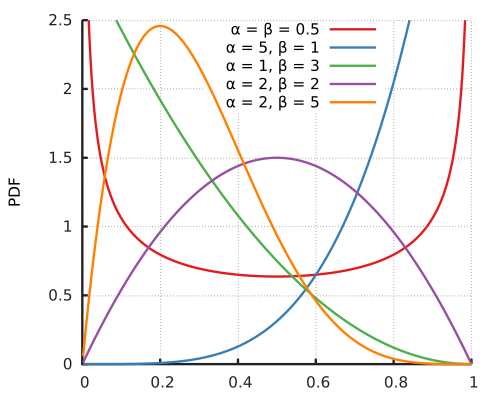
\includegraphics[scale=0.3]{densities/beta}
	}
	\only<3>{
		Gamma
	
		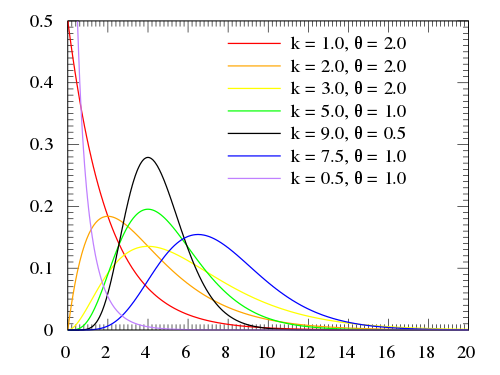
\includegraphics[scale=0.3]{densities/gamma}
	}
	\only<4>{
		Weibull
	
		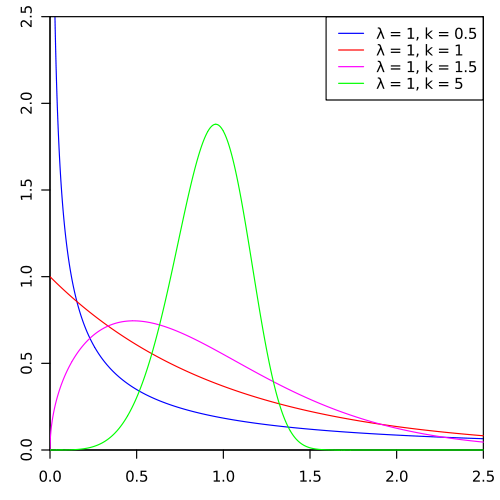
\includegraphics[scale=0.25]{densities/weibull}
	}
	\only<5>{
		Dirichlet
	
		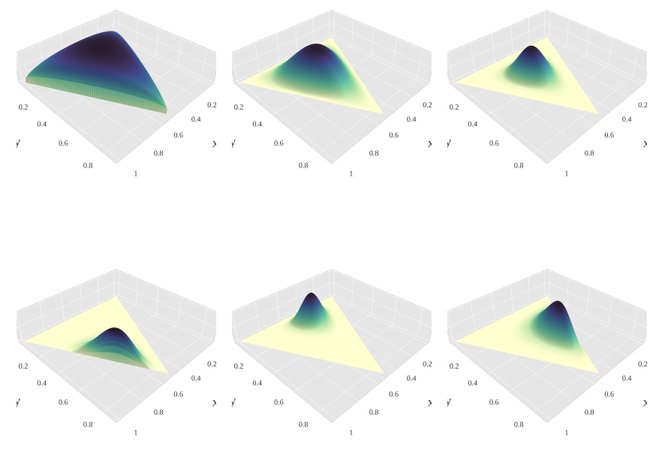
\includegraphics[scale=0.3]{densities/dirichlet}
	}
	\only<6>{
		von Mises-Fisher 
	
		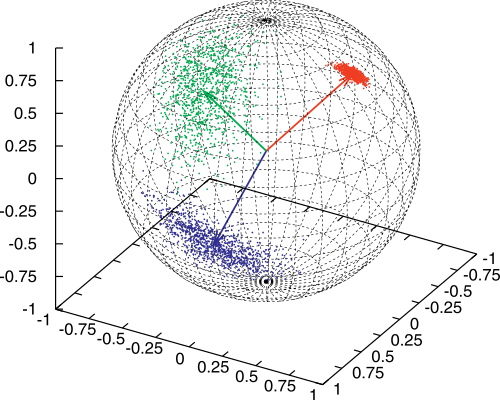
\includegraphics[scale=0.3]{densities/spherical}
	}
	
	%\begin{itemize}
	%	\item e.g. Beta, Gamma, Dirichlet, von Mises-Fisher
	%\end{itemize} 
	%
	%The inverse cdf of a multivariate rv is seldom known in closed-form
	%\begin{itemize}
	%	\item Dirichlet, von Mises-Fisher
	%\end{itemize}

\end{frame}

\section{ADVI}

\begin{frame}{Automatic Differentiation VI}
	Motivation
	\begin{itemize}
		\item many models have intractable posteriors\\
		their normalising constants (evidence) lack analytic solutions \pause
		\item but many models are differentiable\\
		that's the main constraint for using NNs \pause
	\end{itemize}

	Reparameterised gradients are a step towards automatising VI for differentiable models \pause
	\begin{itemize}
		\item but not every model of interest employs rvs for which a reparameterisation is known %standardisation function is known
	\end{itemize}
	
\end{frame}


\begin{frame}{Example: Weibull-Poisson model}
	Suppose we have some ordinal data which we assume to be Poisson-distributed
	\begin{equation*}	
	\begin{aligned}
		\uncover<3->{\alert{z}|r, k &\sim \alert{\Weibull(r, k)}} & \uncover<3->{r \in \mathbb R_{>0}, k \in \mathbb R_{>0}}	\\
		X|\alert{z} &\sim \Poisson(\alert{z}) 
		&\alert{z} \in \mathbb R_{>0}
	\end{aligned}
	\end{equation*}
	\uncover<2->{and suppose we want to impose a Weibull prior on the Poisson rate}
	
	%\alert{FINISH EXAMPLE, GIVE THE OVERVIEW OF ADVI ``PSEUDO-CODE'' FIRST}
	% ALONG THE LINES OF THE "ADVI" SLIDE BUT WITH SIMPLE LANGUAGE
\end{frame}

\begin{frame}{VI for Weibull-Poisson model}
	Generative model
	\begin{equation*}
		\begin{aligned}
			&p(x, z|r,k) = p(z|r, k) p(x|\rho) \pause
		\end{aligned}
	\end{equation*}
	
	Marginal 
	\begin{equation*}
		p(x|r,k) = \int_{\alert{\mathbb R_{>0}}} p(z|r, k) p(x|\rho) \dd z
	\end{equation*}
	
	\pause
	
	ELBO 
	\begin{equation*}
		\E[\alert{q(z|\lambda)}]{\log p(x, z|r,k)} + \Ent{q(z)} \pause
	\end{equation*}
	\alert{Can we make $q(z|\lambda)$ Gaussian?} \\ \pause 
	~ \alert{No! $\supp(\mathcal N(z|\mu, \sigma^2)) = \mathbb R$}
\end{frame}

\begin{frame}{Strategy}

	Build a change of variable into the model 
	\begin{equation*}
		\begin{aligned}
			&p(x, \alert{z}|r,k) = p(\alert{z}|r, k) p(x|\rho) \\
			&= \Weibull(\alert{z}|r, k) \Poisson(x|z) \\ 
			\uncover<2->{&= \Weibull(\underbrace{\uncover<3->{\exp(\galert{\zeta})}}_{\alert{z}}|r, k)  \Poisson(x|\underbrace{\uncover<3->{\exp(\galert{\zeta})}}_{\alert{z}})\uncover<4->{\djac{\exp}{\galert{\zeta}}}  }
		\end{aligned}
	\end{equation*}
	
	\uncover<6->{
	ELBO
	\begin{equation*}
		\E[q(\zeta|\lambda)]{\ldots} + \Ent{q(\zeta)}
	\end{equation*}
	\uncover<7->{
		\alert{Can we use a Gaussian approximate posterior?} \pause \uncover<8->{\galert{Yes!}}
	}
	}

\end{frame}

\begin{frame}{Differentiable models}

	We focus on \emph{differentiable probability models}
	\begin{equation*}
		p(x,z) = p(x|z)p(z)
	\end{equation*}
	\pause
	\begin{itemize}
		\item members of this class have continuous latent variables $z$\\ \pause
		\item and the gradient $\grad_z \log p(x,z)$ is valid within the \emph{support} of the prior 
		$\supp(p(z)) = \{ z \in \mathbb R^K : p(z) > 0 \} \subseteq \mathbb R^K$
	\end{itemize}
	
\end{frame}

\begin{frame}{Why do we need differentiable models?}
	
	Recall the gradient of the ELBO
	\begin{equation*}
		\only<1>{\pdv{\lambda} \E[q(z; \lambda)]{\log p(x,z)}}\only<2->{\alert{\pdv{\lambda} \E[q(z; \lambda)]{\log p(x,z)}}} +  \only<1>{\pdv{\lambda} \Ent{q(z; \lambda)}}\only<2->{\textcolor{gray}{\pdv{\lambda} \Ent{q(z; \lambda)}}} 
	\end{equation*}
	
	\pause
	
	Reparameterisation requires $\pdv{}{z}$
	\uncover<3->{
	\begin{equation*}
	\begin{aligned}
		\pdv{\lambda} \E[q(z; \lambda)]{\log p(x,z)} \uncover<4->{= \E[\pi(\epsilon)]{\pdv{\lambda} \log p(x,z=\inv{\mathcal S}_\lambda(\epsilon))}} \\
		\uncover<5->{= \E[\pi(\epsilon)]{\alert{\pdv{z} \log p(x,z)} \pdv{\lambda} \inv{\mathcal S}_\lambda(\epsilon)}}
	\end{aligned}
	\end{equation*}
	}

\end{frame}

\begin{frame}{VI optimisation problem}
	Let's focus on the design and optimisation of the variational approximation
	\begin{equation*}
		\argmin_{\balert{q(z)}} \KL{\balert{q(z)}}{\alert{p(z|x)}}
	\end{equation*}

	\pause
	
	To automatise the search for a variational approximation $\balert{q(z)}$ we must ensure that\\
	 \begin{equation*}
	 	\supp(\balert{q(z)}) \subseteq \supp(\alert{p(z|x)})
	\end{equation*} \pause
	
	\vspace{-10pt}
	 \begin{itemize}
	 	\item otherwise KL is not a real number\\
		$\KL{q}{p} = \E[q]{\log q} - \E[q]{\log p} \overset{\text{def}}{=} \infty$
	\end{itemize}	
	 
\end{frame}

\begin{frame}{Support matching constraint}

	So let's constrain $q(z)$ to a family $\mathcal Q$ whose support is included in the support of the \alert{posterior}
	 \begin{equation*}
		\argmin_{\balert{q(z)} \in \mathcal Q} \KL{\balert{q(z)}}{\alert{p(z|x)}}
	\end{equation*}
	where
	\begin{equation*}
	 	\mathcal Q = \{\balert{q(z)}: \supp(\balert{q(z)}) \subseteq \supp(\alert{p(z|x)}) \}
	\end{equation*}
	
	\pause
	
	\alert{But what is the support of $\alert{p(z|x)}$?} \pause
	 \begin{itemize}
		\item typically the same as the support of $\galert{p(z)}$\\ \pause
		as long as $p(x,z) > 0$ if $p(z) > 0$		
	 \end{itemize}
	 
\end{frame}

\begin{frame}{Parametric family}

	So let's constrain $q(z)$ to a family $\mathcal Q$ whose support is included in the support of the \galert{prior}
	 \begin{equation*}
		\argmin_{\balert{q(z)} \in \mathcal Q} \KL{\balert{q(z)}}{\alert{p(z|x)}}
	\end{equation*}
	where
	\begin{equation*}
	 	\mathcal Q = \{\balert{q(z; \lambda)}: \lambda \in \Lambda, \supp(\balert{q(z; \lambda)}) \subseteq \supp(\galert{p(z)})  \}
	\end{equation*}
	
	\vspace{-10pt} \pause
	 \begin{itemize}
	 	\item a parameter vector $\lambda$ picks out a member of the family
	\end{itemize}

\end{frame}

\begin{frame}{Constrained optimisation for the ELBO}

	We maximise the ELBO 
	\begin{equation*}
		\argmax_{\lambda \in \Lambda} \E[\balert{q(z; \lambda)}]{\log p(x, z)} + \Ent{\balert{q(z; \lambda)}}
	\end{equation*}
	\pause subject to
	 \begin{equation*}
		\mathcal Q = \{\balert{q(z; \lambda)}: \lambda \in \Lambda, \supp(\balert{q(z; \lambda)}) \subseteq \supp(\galert{p(z)})  \}
	\end{equation*}
	\pause
	
	\vspace{-10pt}
	Often there can be two constraints here\pause
	\begin{itemize}
		\item \galert{support matching constraint} \pause
		\item \alert{$\Lambda$ may be constrained to a subset of $\mathbb R^D$}\\ \pause
		e.g. univariate Gaussian location lives in $\mathbb R$ but scale lives in $\mathbb R_{>0}$
	\end{itemize}

\end{frame}

\begin{frame}{Parameters in real coordinate space}
	
	Consider the Gaussian case: $Z \sim \mathcal N(\mu, \sigma)$ \\ \pause
	~ how can we obtain $\mu \in \mathbb R^d$ and $\sigma \in \mathbb R^d_{\alert{>0}}$ \\
	~ from $\lambda_\mu \in \mathbb R^d$ and $\lambda_\sigma \in \mathbb R^d$? \pause
	\begin{itemize}
		\item $\mu = \lambda_\mu$ \pause
		\item $\sigma = \galert{\exp}(\lambda_\sigma)$ \pause or $\sigma = \galert{\softplus}(\lambda_\sigma)$ 
	\end{itemize}
	
	\pause
	
	The vMF distribution is parameterised by a unit-norm vector $v$\\
	~ how can we get $v$ from $\lambda_v \in \mathbb R^d$? \pause
	\begin{itemize}
		\item $v = \galert{\frac{\textcolor{black}{\lambda_v}}{\norm{\textcolor{black}{\lambda_v}}_2}}$  \pause
	\end{itemize}
	
	It is typically possible to work with unconstrained parameters, \galert{it only takes an appropriate activation}
	
	
\end{frame}


\begin{frame}{Constrained optimisation for the ELBO}

	We maximise the ELBO 
	\begin{equation*}
		\argmax_{\lambda \in \galert{\mathbb R^D}} \E[\balert{q(z; \lambda)}]{\log p(x, z)} + \Ent{\balert{q(z; \lambda)}}
	\end{equation*}
	\pause 	subject to
	 \begin{equation*}
		\mathcal Q = \{\balert{q(z; \lambda)}: \lambda \in \galert{\mathbb R^D}, \supp(\balert{q(z; \lambda)}) \subseteq \alert{\supp(p(z))}  \}
	\end{equation*}
	
	\vspace{-10pt}
	There is one constraint left\pause
	\begin{itemize}
		\item \alert{support of $q(z; \lambda)$ depends on the choice of prior}\looseness=-1 \\
		\alert{and thus may be a subset of $\mathbb R^K$}
	\end{itemize}

\end{frame}

\begin{frame}{ADVI}
	
	A gradient-based black-box VI procedure \pause
	\begin{enumerate}		
		\item \alert{Custom parameter space} \pause
			\begin{itemize}
				\item \galert{Appropriate transformations of unconstrained parameters!} \pause
			\end{itemize}
		\item \alert{Custom $\supp(p(z))$} \pause
			\begin{itemize}
				\item \galert{Express $z \in \supp(p(z)) \subseteq \mathbb R^K$ as a transformation of some unconstrained $\zeta \in \mathbb R^K$} \pause
				\item \galert{Pick a variational family over the entire real coordinate space} \pause
				\item \galert{basically, pick a Gaussian!} \pause
				%\item \galert{And pick one for which a standardisation exists!} \pause
			\end{itemize}
		\item \alert{Intractable expectations} \pause
			\begin{itemize}
				\item \galert{Reparameterised Gradients!} 
			\end{itemize}
	\end{enumerate}
		
\end{frame}

\begin{frame}{Joint model in real coordinate space}

	Let's introduce an invertible and differentiable transformation
	\begin{equation*}
		\mathcal T: \supp(p(z)) \to \mathbb R^K
	\end{equation*} \pause
	 and define a transformed variable $\zeta \in \mathbb R^K$
	\begin{equation*}
		\zeta = \mathcal T(z)
 	\end{equation*} \pause
	
	\vspace{-10pt}	
	
	Recall that we have a joint density $p(x,z)$\\ \pause
	~ which we can use to construct $p(x, \zeta)$ \pause
	\begin{equation*}
		p(x, \zeta) = p(x, \underbrace{\uncover<6->{\inv{\mathcal T}(\zeta)}}_{z}) \djac{\uncover<7->{\inv{\mathcal T}}}{\uncover<7->{\zeta}}
	\end{equation*}
	
\end{frame}

\begin{frame}{VI in real coordinate space}
	We can design a posterior approximation whose support is $\mathbb R^K$\\ \pause
	
	\begin{equation*}
	\begin{aligned}
		q(\zeta; \lambda) \pause &= \underbrace{\galert{\prod_{k=1}^K} q(\zeta_{\galert{k}}; \lambda)}_{\text{mean field}} \pause
		&= \prod_{k=1}^K \galert{\mathcal N(\zeta_k|\mu_k, \sigma^2_k)} \\ 
	\end{aligned}
	\end{equation*}
	where
	\begin{itemize}
		\item $\mu_k = \lambda_{\mu_k}$ for $\lambda_{\mu_k} \in \mathbb R^K$
		\item $\sigma_k = \softplus(\lambda_{\sigma_k})$ for $\lambda_{\sigma_k} \in \mathbb R^K$
	\end{itemize}
	
\end{frame}


\begin{frame}{ELBO in real coordinate space}
\Wider[4em]{	
	\begin{equation*}
	\begin{aligned}
		&\log p(x) \pause = \log \int p(x,\alert{z}) \dd \alert{z}  \\ \pause
		&= \log \int p(x,\alert{\inv{\mathcal T}(\zeta)}) \alert{\djac{\inv{\mathcal T}}{\zeta} \dd \zeta}	\\	\pause
		&= \log \int \galert{q(\zeta)} \frac{p(x,\inv{\mathcal T}(\zeta)) \djac{\inv{\mathcal T}}{\zeta}}{\galert{q(\zeta)}} \dd \zeta \\ \pause
		&\overset{\text{JI}}{\alert{\ge}}  \int q(\zeta) \alert{\log} \frac{p(x,\inv{\mathcal T}(\zeta)) \djac{\inv{\mathcal T}}{\zeta}}{q(\zeta)} \dd \zeta \\ \pause
		&= \E[q(\zeta)]{\log p(x,\inv{\mathcal T}(\zeta)) + \log \djac{\inv{\mathcal T}}{\zeta}} + \Ent{q(\zeta)}
	\end{aligned}
	\end{equation*}
}
\end{frame}

\begin{frame}{Reparameterised ELBO}
	
	Recall that for Gaussians we have a standardisation procedure $\mathcal S_\lambda(\zeta) \sim \mathcal N(\epsilon| 0, I)$
	

	\begin{small}
	\begin{equation*}
	\begin{aligned}
		&\alert{\E[q(\zeta; \lambda)]{\log p(x, \inv{\mathcal T}(\zeta)) + \log \djac{\inv{\mathcal T}}{\zeta}}} + \galert{\Ent{q(\zeta; \lambda)}}  \\ \pause
		&= \E[\mathcal N(\epsilon|0, I)]{\log p(x, \underbrace{\inv{\mathcal T}(\overbrace{\inv{\mathcal S}_\lambda(\epsilon)}^{\zeta})}_{z}) + \log \djac{\inv{\mathcal T}}{\inv{\mathcal S}_\lambda(\epsilon)} } \\
		&+ \Ent{q(\zeta; \lambda)}
	\end{aligned}
	\end{equation*}
	\end{small}

\end{frame}

\begin{frame}{Gradient estimate}

	
	\begin{small}
	For $\epsilon_i \sim \mathcal N(0, I)$
	
	\begin{equation*}
		\begin{aligned}
		\pdv{\lambda}\ELBO(\lambda) \pause \overset{\text{MC}}{\approx}& \frac{1}{M} \sum_{i=1}^M \pdv{\lambda} \log \underbrace{p(x|\inv{\mathcal T}(\inv{\mathcal S}_\lambda(\epsilon_i)))}_{\text{likelihood}} \\ \pause
		&\phantom{\frac{1}{M} \sum}+ \pdv{\lambda} \log \underbrace{p(\inv{\mathcal T}(\inv{\mathcal S}_\lambda(\epsilon_i)))}_{\text{prior}} \\ \pause
		&\phantom{\frac{1}{M} \sum}+ \pdv{\lambda} \log \underbrace{\djac{\inv{\mathcal T}}{\inv{\mathcal S}_\lambda(\epsilon_i)}}_{\text{change of volume}} \\ \pause
		&+ \pdv{\lambda} \underbrace{\Ent{q(\zeta; \lambda)}}_{\text{analaytic}}
		\end{aligned}
	\end{equation*}
	
	\end{small}

\end{frame}

\begin{frame}{Practical tips}

	Many software packages know how to transform the support of various distributions
	\begin{itemize}
		\item Stan
		\item Tensorflow \texttt{tf.probability}
		\item Pytorch \texttt{torch.distributions}
	\end{itemize}
\end{frame}

\section{Example}


\begin{frame}{Weibull-Poisson model}

	Build a change of variable into the model 
	\begin{small}
	\begin{equation*}
		\begin{aligned}
			&p(x, \alert{z}|r,k) = p(\alert{z}|r, k) p(x|\rho) \\
			&= \Weibull(\alert{z}|r, k) \Poisson(x|z) \\ 
			\uncover<2->{&= \Weibull(\underbrace{\uncover<3->{\inv{\log}(\galert{\zeta})}}_{\alert{z}}|r, k)  \Poisson(x|\underbrace{\uncover<3->{\inv{\log}(\galert{\zeta})}}_{\alert{z}})\uncover<4->{\djac{\inv{\log}}{\galert{\zeta}}}  } \\
			\uncover<5->{&= p(x, \alert{z} = \inv{\log}(\galert{\zeta})) \djac{\inv{\log}}{\galert{\zeta}}}
		\end{aligned}
	\end{equation*}
	\end{small}
	
	\uncover<6->{
	ELBO
	\begin{small}
	\begin{equation*}
	\begin{aligned}
		&\E[q(\zeta|\lambda)]{\only<6>{\ldots}\only<7->{\log p(x, z = \inv{\log}(\zeta)) \djac{\inv{\log}}{\zeta}}} + \Ent{q(\zeta)} \\
		&\uncover<8->{\E[\phi(\epsilon)]{\log p(x, z = \inv{\log}(\inv{\mathcal S}(\epsilon))) \djac{\inv{\log}}{\inv{\mathcal S}(\epsilon)}} + \Ent{q(\zeta)} }
	\end{aligned}
	\end{equation*}
	\end{small}
	
	}

\end{frame}

\begin{frame}{Visualisation}

	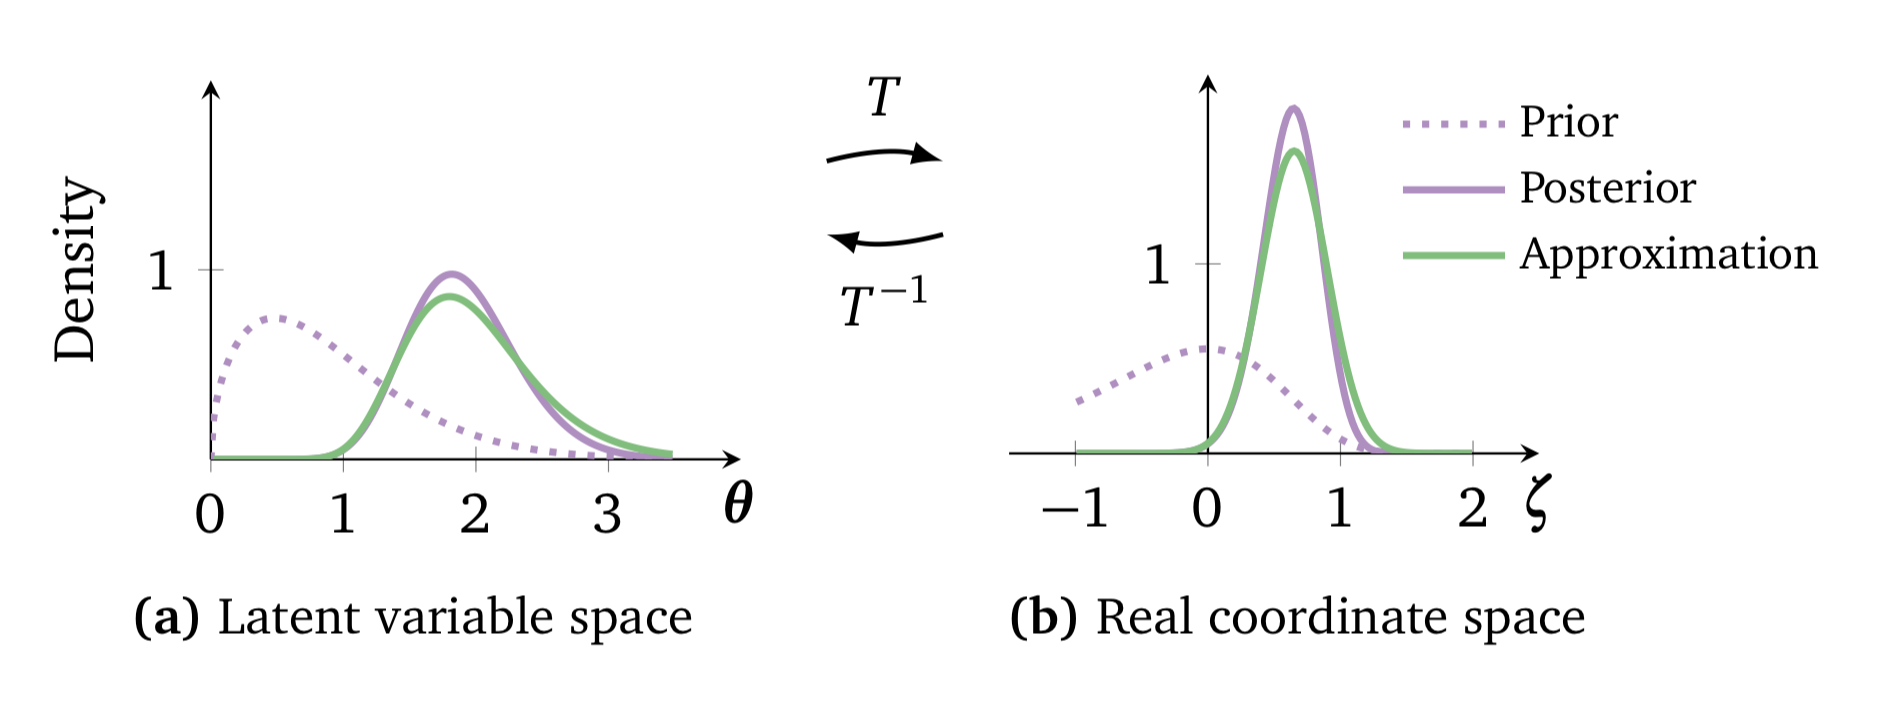
\includegraphics[scale=0.25]{advi/t} 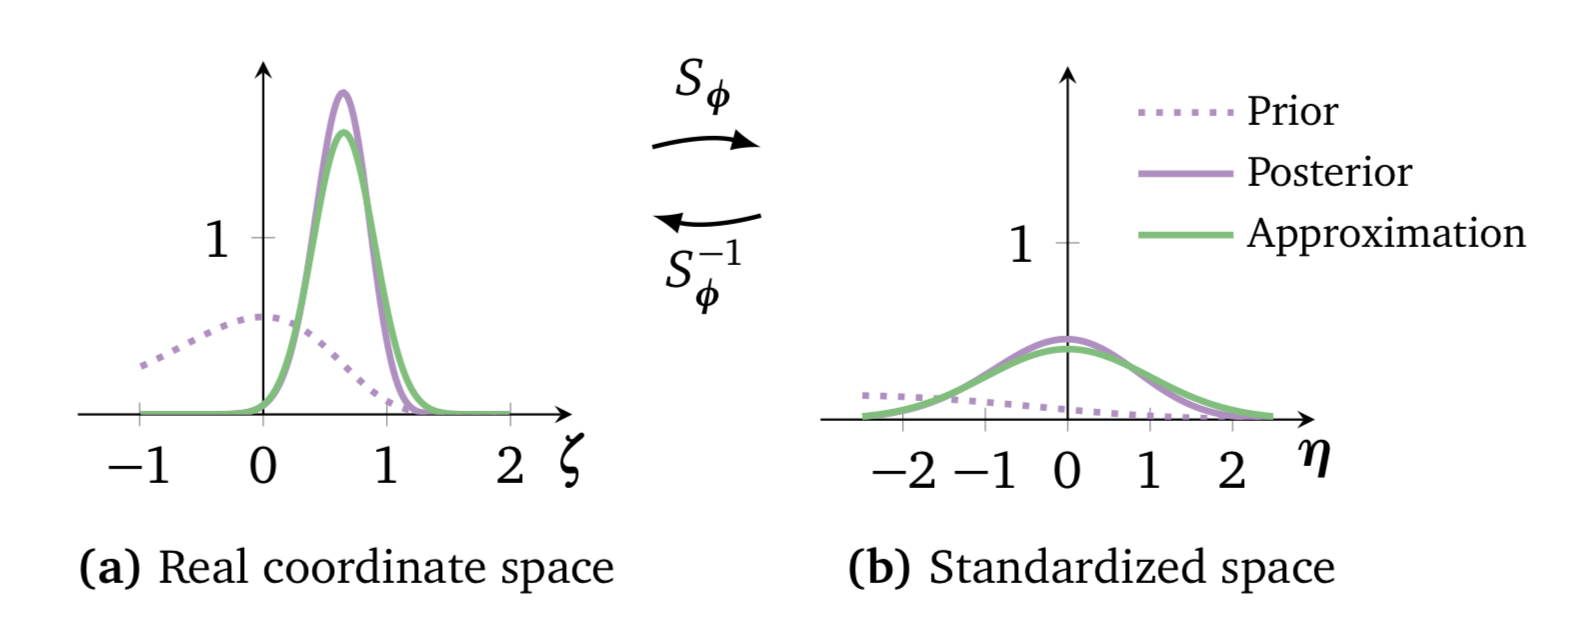
\includegraphics[scale=0.3]{advi/s}
	
	Images from \citet{KucukelbirEtAl:2017}
\end{frame}


\begin{frame}{Wait... no deep learning?}

	Sure! Parameters may well be predicted by NNs
	
	\begin{itemize}
		\item approximate posterior location and scale
		\item Weibull rate and shape
	\end{itemize}
	
	Everything is now differentiable, reparameterisable, and the optimisation is unconstrained!
	
\end{frame}


\begin{frame}{Summary}

ADVI is a big step towards blackbox VI \pause
\begin{itemize}
	\item we knew how to map parameters to the unconstrained real coordinate space \pause
	\item now we also know how to map latent variables to unconstrained real coordinate space \pause
	\item it takes a change of variable built into the model \pause
\end{itemize}

Think of ADVI as reparameterised gradients and autodiff expanded to many more models! \pause

\alert{What's left?} \pause Our posteriors are still rather simple, aren't they?

\end{frame}


\begin{frame}[allowframebreaks]
\bibliographystyle{plainnat}
\bibliography{../../VI}
\end{frame}


\end{document}